\cleardoublepage
\counterwithout{figure}{section}
\counterwithout{table}{section} 
\counterwithout{equation}{section}
\counterwithin{figure}{chapter}
\counterwithin{table}{chapter} 
\counterwithin{equation}{chapter}


\chapter{Introduction}
\label{sec:problemstellung}
 Only in Germany more than 1 Million teeth are replaced annually. The replacement procedure is accomplished with an implantation of the tooth replica to provide the aesthetics and the function of the natural tooth. Ancient Egyptians used tooth shaped ivory to regain the function of the missing teeth. Today the technology has evolved to a point where the dental replacement for a single tooth is an assembly of three parts, which  are to be seen in Figure 1.1. The implant is the part which is screwed to the lower jaw bone (mandible) and anchors the whole replacement assembly to the chin. The preferred material used for the implant are titanium in the EU and tantalum in the US. The enhanced osseointegration of the porous implant material surface, biocompatibility of the ceramic interface, formed due to the surface oxidation a Young's Modulus, which is similar to the human bone are the main reasons for titanium and tantalum to be the prime materials for this purpose. The abutment takes on the task of a fitting  for the crown and is made of the same material as the implant.
  \begin{figure}[h]
 	\centering
 	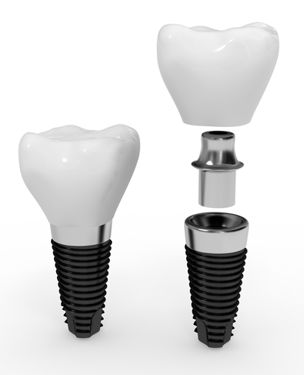
\includegraphics[width=0.4\textwidth]{grafiken/implant.png}
 	\caption{Single tooth replacement}
 	\label{fig:implant}
 \end{figure} 
 
 The crown of the tooth replacement is the part which imitates the visual qualities of the tooth. There are several material, which a crown can be made of or assembled from. The most popular crown material dominating the market is the Yttria-stabilized zirconia (YSZ), which has a cubic fluorite crystal structure and is going to be referred as zirconia in the frame of this thesis. However, zirconia in its pure form is a plain white material with high translucency. In case of single tooth replacement  the newle implanted crown would be absurdly white when compared to the neighboring teeth.Even when a full chin dental replacement is conducted, it is abnormal to have a full set of plain white teeth without any shading. This situation makes it a necessity to preprocess the crowns to match the neighboring teeth or another natural shade of choice in case of a fully monolithic replacement. Dentist are using a shade guide seen in the figure \ref{fig:shadeguide} for a side-by-side comparison to determine the color and the shade of the teeth. One can observe that there are 4 color groups A, B, C and D which are referred as orange-brown, yellow, grey-brown and red respectively \citep{vita}. Each of these colors have shades ranging from 1 to 4. Even though the shades are coded with the numbers from 1 to 4 with increments of 0.5 a total analogue shade acquisition is possible. The number 1 represents the shade with the least and 4 with the most saturated tone for each color.
 \newline
 \begin{figure}[h]
 	\centering
 	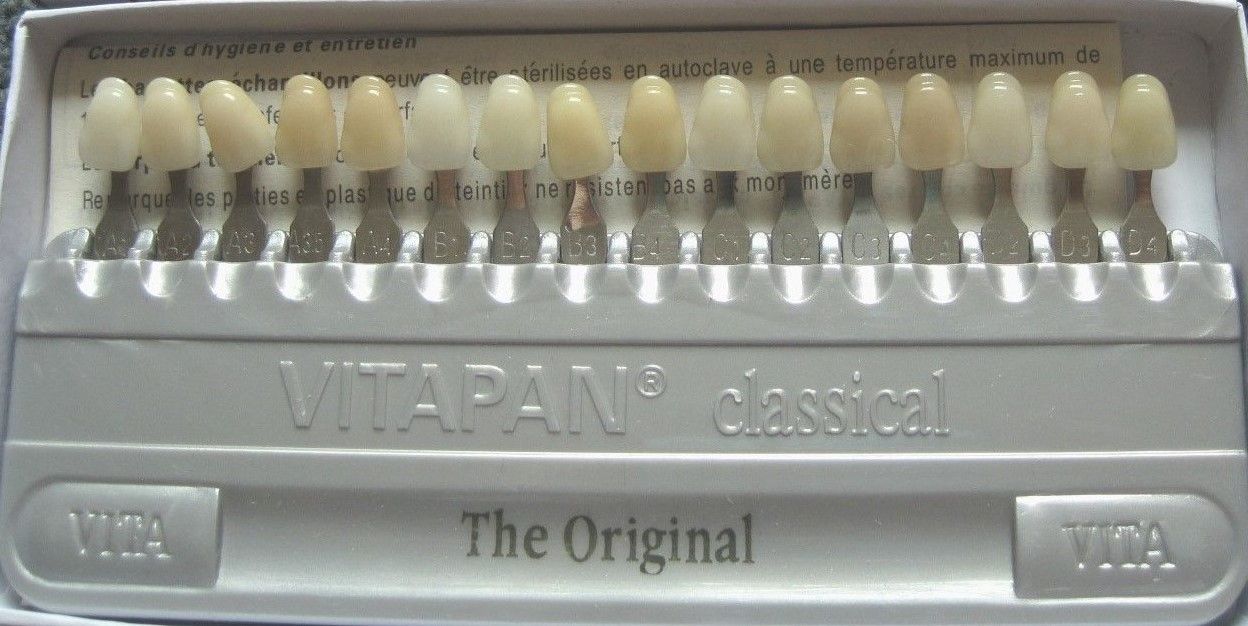
\includegraphics[width=0.9\textwidth]{grafiken/shadeguide.jpg}
 	\caption{Vitapan Shadeguide}
 	\label{fig:shadeguide}
 \end{figure}  
 


\chapter{State of the Research}
\label{sec:stand_forschung}

Addressing the shading process of the dental zirconia-based ceramics as a combined procedure of drop generation, dispersion of the ink within the porous material and post sintering generation of the color below the surface of the porous material, it can be said that the quantitative coloring process of the dental crowns is an uncharted area for the scientific researches in the present-day. 


In 2016 Lee et al. have investigated the absorption behavior of water drops impinging porous stones experimentally and numerically. The investigation includes the phases from spreading to evaporation for a water droplet considering the absorbed amount of the droplet during the depletion and spreading of the humidity within the manner depending on time for three porous materials. Quantitative measurements of the water absorption for the materials are conducted with high-speed imaging and neutron radiography methods during the time range from the impact moment to the end of the spreading phase after absorption. Neutron radiography shows a high resolution quantitative distribution of absorbed water. During the first contact and deposition on the surface the droplets do not exhibit a wetting behavior.  As soon as the droplet acquires its maximum diameter on the surface, it gets fixed and the contact angle with the surface remains constant as long as the droplet is not drained by the stone. The absorption behavior doesn’t have the same attributes throughout the whole process. At the beginning the material shows a contact resistance blocking the absorption, which is associated with the entrapped air beneath the area encapsulated by the borders of the water droplet. In the second phase the encapsulated air finds a way to diffuse away so the capillary flow takes place flawlessly until the total disappearance of the droplet on the surface is observed. The experimental data shows accordance to the phases of the numerical model for water flow inside the unsaturated porous material. The collision velocity has a huge effect on drop spreading on the surface and impregnation, but not so much on the distribution of the water after the initial absorption. The absorption and distribution rates are highly relevant to the capillary structure of the stones.\citep{lee2016absorption}

On a different aspect some research has been conducted about the effect of the coloring process on the structural strength of the zirconia. In the research of Shah et al. coloring zirconia with cerium acetate mixtures with a maximum ink weight ratio of 5\% provided a distinctive shade and did not cause a mechanical disadvantage. However, the ratios above 5\% have decreased the mechanical properties while not increasing the shading level significantly. The paper also includes data for case where the coloring process is conducted using cerium chloride and bismuth chloride. For both cases 1\% coloring agent was the limit, if the flexural strength was to be conserved. The low temperature degradation was also observed in the frame of the paper, which did not show any co-dependence with the coloring solution.\citep{shah2008effect}


The crystallographic state of zirconia depends on the temperature under atmospheric pressure. Until reaching a temperature of {1170\textdegree} Celcius the crystallographic structure shows a monoclinic symmetry. After that temperature the structure can be defined as tetragonal until {2370\textdegree} C , which afterwards becomes cubic up to the melting point. The volume of the material increases about 4.5\% during the transformation from tetragonal to monoclinic phases, which is enough to cause a crack induced failure. This evitable transformation begins at about {950\textdegree} C while cooling down and the only way to stabilize the tetragonal structure is creating CaO, MgO, $Y_{2}O_{3}$ or $CeO_{2}$ oxides inside the structure to keep the tetragonal formation  at room temperature, which eliminates the crack induction and therefore the structural failure of the material parallel to an enhanced toughness. \citep{denry2008state}

Pecho et al. have conducted experiments to analyse the optical behaviour of dental zirconia and dentin in comparison utilizing Kubelka-Munk theory. The results show that the current zirconia materials alone could not satisfy the luminous transmittance of the natural dentin so an additive application of masking is required to reach an approximate to the natural tooth.\citep{pecho2015optical}

The infiltration time of the porous medium was formulated by Markicevic et al. in 2009 as:

\begin{equation}
t_{in}=\kappa \cdotp {\frac{\mu \cdotp r{_0}^{1.85}}{\sigma \cos({\theta})\varPhi^{0.38}}}
\end{equation}
\newline
$t_{in}$ defines the infiltration time and depends on the parameters $\kappa$ , which is the permeability constant of the medium and $\mu$ the kinematic viscosity of the fluid. The initial drop radius is symbolized by $r_{0}$. $\theta$ stands for the initial contact angle after the impact of the droplet on the surface. The $\sigma$ in the denominator is the surface tension of the liquid. The higher the surface tension is the harder it is for the liquid to wet the surface of the material because of the increased contact angle and hardened impregnation capability. The last dependency of the infiltration time is  the $\phi$ constant for the material, identifying the porosity level of the material. \citep{markicevic2009infiltration}

Stratov et al. have provided experimental results regarding  the spreading phases of silicon oil droplets utilizing capillary forces over different permeable layers and observing the diameters of the droplets and wetted areas over time. They have divided the depletion into two phases, of which the first one is defined by the time to reach the maximum diameter for the drop base and the second one is identified by the reduction of the drop base while the depletion takes place. The findings of the experiments show that the different oils on the different porous material with similar porosity and mean pore dimensions. showed similar spreading characteristics on a different time scale and the contact angle remained constant throughout the second stage.\citep{starov2002thick}

The dispersion behavior of liquid drops inside porous media which are previously saturated with the identical liquid are examined in the work of Starov et al. The study was conducted considering both theoretical and experimental perspectives. The study was conducted both theoretical and experimental perspectives. The spreading of a liquid on a dry solid medium is governed by a power law and it is shown that the same power law applies to the case with saturated medium. The liquid flow within the porous medium is modeled using the Brinkman’s equations. The effective lubrication and the liquid exchange between the drop and the porous medium are found to have equal significance through which the drop dispersion equation is generated. \citep{starov2002saturated}
\newline

\begin{equation}
L=L_0 (1+10(\frac{4}{\pi})^3 \frac{V^3 \gamma}{L_0^{10} \mu}\omega t)^{0.1}
\end{equation}
\newline

The formula 2.2 shows the parameters which define the diameter of the covered spot by a deployed drop on the saturated surface of the porous material. $L_0$ V are the measured initial diameter and volume of the drop. $\omega$ is defined as the effective lubrication coefficient and has to be acquired experimentally for each porous medium and impregnating liquid pair. The t as the last parameter of the equation stands for the time as usual. 

The properties of the porous medium, such as its porosity, the size and the orientation of the pores and the chemical properties of the surface affect the impregnation and the dispersion behavior of the drops. The Washburn equation is employed by multiple authors to generate a model. These models are grounded on the existence of cylindrical capillaries lying parallel to each other. The Washburn equation describes the behavior of the drops by stating that the wetting is induced bu capillary pressure while the viscous dissipation of the flow causes resistance to the dissipation.

The amount of time it takes for a drop to diffuse completely in the porous substrate, until there remains no more liquid on the surface is defined as the drop penetration time, also called as the wicking time.

\section{Drop Deployment}


\subsection{Piezoelectric}


\subsection{Electromagnetic}
\label{sec:freiheitsgrad_eines_getriebes}


\section{Ceramic coloring}
\label{sec:grundlagen_für_die_kinematischen_betrachtungen}


\chapter{State of the Technology}
\label{sec:stand_technik}
Even in the most contemporary dental laboratory of today's world, the coloring process is accomplished manually by a experienced dental technologist, who is following the guidelines prepared by the dental ink companies, which explain how a dental crown has to be colored sequentially using different colors on different areas of a single crown summarized in about 20 basic steps. The application of the ink on the dental crown with brush strokes takes about 5 minutes for each tooth depending on the manual measurements of the ink application process conducted by a dental technologist from Zirkonzahn for educational purposes.
On the left side you can see a cutout of a lab card. Dentists mark different areas of the crown with different colors from the guide for the technicians.
And on the right side are the tasks of a dental technician, which are mainly. Milling, Manually coloring using a brush, furnacing to burn the color to the zirconia and lastly polishing for a natural look.
And the coloring part is the process, on which this thesis is focused.
\begin{figure}[h]
	\centering
	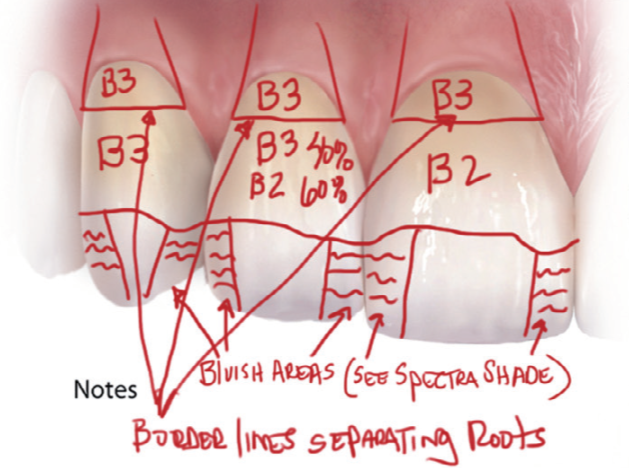
\includegraphics[width=0.5\textwidth]{grafiken/lab_card.png}
			\caption{Cutout of a lab card \citep{sharpling2014}}
	\label{fig:lab_card}
\end{figure}

\begin{figure}[h]
	\centering
	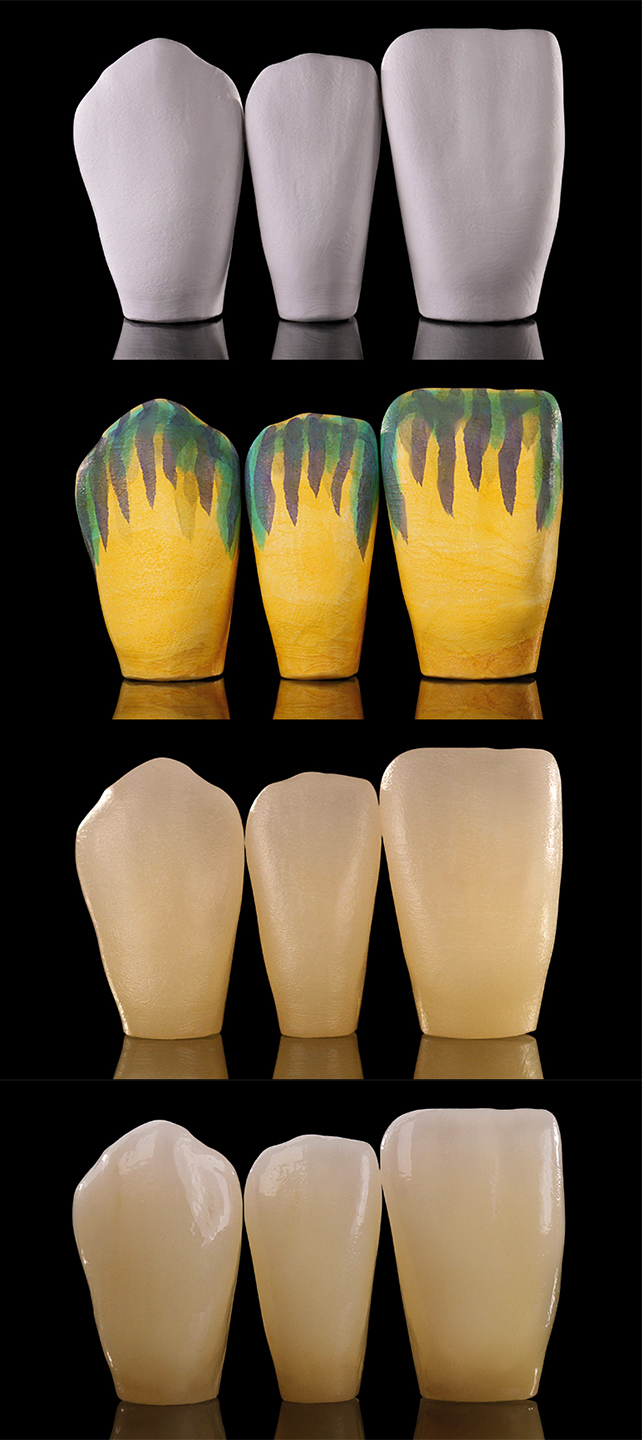
\includegraphics[height=0.6\textwidth]{grafiken/CrownProcesses.jpg}
	\caption{Making of dental implants \citep{zirkonzahn2018} }
	\label{fig:CrownProcesses}
\end{figure} 

\begin{figure}[h]
	\centering
	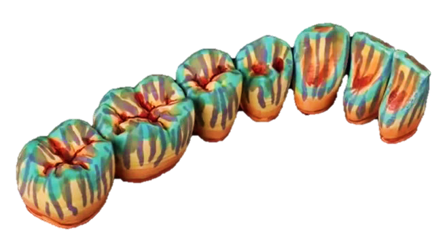
\includegraphics[width=0.6\textwidth]{grafiken/false_colored.png}
	\caption{False colored crowns after manual brushing \citep{zirkonzahn2018}}
	\label{fig:false_colored}
\end{figure}


\chapter{Review of the State of the Art and Technology}
\label{sec:kritik_stand_technik}
